\documentclass[conference]{IEEEtran}
\IEEEoverridecommandlockouts
\usepackage{cite}
\usepackage{amsmath,amssymb}
\usepackage{fontspec}
\setmainfont{texgyretermes}[Extension=.otf, UprightFont=*-regular, BoldFont=*-bold,
  ItalicFont=*-italic, BoldItalicFont=*-bolditalic]
\setmonofont{texgyrecursor}[Extension=.otf, UprightFont=*-regular, BoldFont=*-bold,
  ItalicFont=*-italic, BoldItalicFont=*-bolditalic]
\usepackage{graphicx}
\usepackage{booktabs}
\usepackage{array}
\usepackage{url}
\usepackage{tikz}
\usetikzlibrary{positioning,arrows.meta,fit,backgrounds,calc}
\renewcommand{\arraystretch}{1.1}
\def\UrlBreaks{\do\/\do-\do.\do\#}

\begin{document}

\title{Privacy-Preserving Context-Aware Password Risk Assessment with Cross-Account Dependency Analysis and Save-Time Intervention}

\author{\IEEEauthorblockN{Jasmeet Ranjan Srivastava, Garvit Singla, Rakshit Kapoor}
\IEEEauthorblockA{[Affiliation to be added]}}

\maketitle

\begin{abstract}
A password can be structurally complex and still be predictable from its owner's personal details or from the owner's other passwords. Password managers protect stored credentials, but they rarely assess these relationships or act before a risky password is stored. This paper presents the Context-Aware Local Vault (CAV), a local-first password manager. Its assessment combines breach evidence obtained through a k-anonymity range query, coverage of personal attributes that the user declares, structural weakness estimated by zxcvbn, exact reuse and derivative-password families. These signals feed a criticality-weighted Vault Health Score. Password age is retained only as an optional policy input. An unavailable breach check is treated as missing evidence and produces a score interval rather than an assumed value. A save-time gate offers editing, overriding or a locally generated passphrase. Credentials and the personal profile are encrypted under an Argon2id-protected AES-256-GCM key hierarchy, and no remote language model is used. We evaluate the implementation on a synthetic, leakage-checked fixture of 11,022 examples from 1,002 fictional profiles, with a bounded attacker under five knowledge scenarios. On held-out data the personal-context detector reached a precision of 0.989 and a recall of 0.877, but it recovered only 5 of 334 unseen transformations. Against the combined attacker at 1,000 guesses, the fixed-weight score reached a recall of 0.153 at a validation-selected false-positive limit of 5\%, while a logistic baseline on the same features reached 0.503. All 102 automated tests pass. No human-subject results are reported. A four-condition study interface is provided for future work. The results come from synthetic data and do not establish external validity.
\end{abstract}

\begin{IEEEkeywords}
Password management, personal context, targeted password guessing, derivative passwords, k-anonymity, envelope encryption, save-time intervention.
\end{IEEEkeywords}

\section{Introduction}
Passwords remain a common way to prove identity online, and password managers and two-factor tools are the usual response to their weaknesses~\cite{jubur}. Two problems persist. First, people reuse passwords across work and personal accounts~\cite{aiswarya}, so one exposed credential can open several services~\cite{farcasin}. Second, people build passwords from things they know about themselves, such as names, hometowns and birth years. These details are often easy to find in public profiles~\cite{atzori2024}. Composition rules do not reliably improve resistance to cracking~\cite{he}, and rigid policies increase the burden on users, who respond with insecure coping strategies~\cite{umejiaku2023}. AI-assisted, multi-component assessment has precedent in other security domains~\cite{nebbione}. Targeted attacks that combine personal information with a user's old passwords are well established~\cite{ou2026,mdiguess}.

Existing meters address part of this problem. zxcvbn estimates guessing effort from patterns, dictionary terms and keyboard walks~\cite{wheeler}, but it does not check whether a password appears in breach data or whether it is built from the owner's personal details. Saint-Jean et al. reported that structural strength and breach exposure are nearly uncorrelated and proposed combining them~\cite{saintjean}. Personal-context assessment~\cite{atzori2024,alatawi} and multi-source targeted guessing~\cite{mdiguess} already exist, so integrating them is not novel in itself. The question we examine is narrower: whether a local assessment that also uses relationships between the credentials in one vault adds measurable detection value, and whether acting before a password is stored can be studied in a controlled way.

We address four research questions. \textbf{RQ1:} Does locally declared personal context improve attack-relevant detection relative to conventional strength estimation at a controlled false-positive rate? \textbf{RQ2:} Do cross-account relationships improve detection under history-aware attackers, and what does transitive clustering cost? \textbf{RQ3:} Does pre-save feedback reduce vulnerable retained credentials relative to equivalent post-save feedback, and does an immediate alternative add benefit? \textbf{RQ4:} Can these behaviours be delivered with acceptable local privacy exposure and computational overhead? This paper answers RQ1, RQ2 and RQ4 only on synthetic data, and provides the instrument for RQ3 without human results.

The contributions are as follows.
\begin{enumerate}
\item A local assessment that keeps breach evidence, personal-context coverage, structural weakness, exact reuse and derivative relationships as separate signals. Unknown breach status is propagated as a score interval, and age is an opt-in policy input.
\item A save-time gate with three explicit actions and offline passphrase generation, and an isolated four-condition interface (conventional, post-save, pre-save, and pre-save with an alternative) for studying intervention timing.
\item An encrypted vault in which both credentials and the personal profile are AES-256-GCM ciphertext. Breach checks send a five-character hash prefix, and credential suggestions are generated locally. These are established mechanisms, not a new cryptographic contribution.
\item A reproducible evaluation harness with a leakage-checked data contract, a five-scenario bounded attacker, matched baselines and ablations, calibration bands, a security test matrix and local performance measurements. Negative results are reported alongside positive ones.
\end{enumerate}

\section{Related Work}
\textbf{Strength estimation and breach exposure.} Early composition policies counted character classes. Modern meters estimate guessing effort from patterns~\cite{wheeler}. Probabilistic context-free grammars model password structure from breach corpora, and PCFG-based cracking was formalized by Weir et al.~\cite{weir}. Breach exposure is a separate dimension. Saint-Jean et al. proposed $E_{\text{final}}=\min(E_{\text{base}},E_{\text{breach}})$ to capture high-entropy breached passwords~\cite{saintjean}. NIST guidance favours length and blocklist screening over composition rules and periodic changes~\cite{nist63b4}. CAV follows that direction but keeps breach status, structure and personal context as separate signals rather than collapsing them into a single minimum.

\textbf{Neural and data-driven guessing.} Recurrent models have been applied to password and passphrase guessing~\cite{nosenko}. Sun~\cite{sun} proposed a hybrid ResCNN-BiGRU-GAP model that classifies the origin of a password, reporting an F1-macro of 0.952 on that task. Xu et al.~\cite{xu} showed that client-side strength meters built from data-driven models can leak training data through membership inference. This motivates keeping strength evaluation on the device and avoiding distribution of trained models. CAV's live checks are rule-based and lookup-based. A logistic model is fitted only as a research baseline and is never loaded by the application.

\textbf{Personal context and targeted guessing.} SODA ADVANCE reconstructs biographical profiles from social networks and scores passwords against them using CUPP-style dictionaries, leetspeak decoding and coverage metrics~\cite{atzori2024,atzori2025}. G\"uven et al.~\cite{guven} showed that users with multiple breached accounts follow predictable mutation patterns. Ou et al.~\cite{ou2026} combined personally identifiable information with old passwords for targeted guessing, and MDIGuess~\cite{mdiguess} jointly exploits historical passwords, personal information and general leaked-password data. Cipher-Guard~\cite{alatawi} adds context to a machine-learning password assessment. CAV keeps the coverage and leetspeak ideas but replaces scraping with fields that the user declares, so no third-party profile data is collected. Our bounded attacker is a simple deterministic generator. It is not a reproduction of these attacks, and their reported metrics are not comparable with ours.

\textbf{Language models and passwords.} Honeyword systems place decoy passwords beside real ones to detect database theft, and deep learning has been used to separate honeywords from real passwords~\cite{dani}. LLM-based honeyword generation~\cite{umejiaku2025} and LLM password generation~\cite{kagnici} show both defensive uses and predictability risks, and LLMs can also support targeted social engineering~\cite{sai}. An earlier CAV design asked a hosted model for passphrases. Its output did not reliably meet the prompt's constraints, and model output provides no verifiable generation entropy. The current build therefore generates all suggestions locally.

\textbf{Nudging and intervention timing.} A PRISMA-based review of cybersecurity nudges identified informational, default, framing and social nudges, and it reported that feedback and effort-reduction designs produced the most durable effects~\cite{arciulo}. Protection Motivation Theory separates threat appraisal from coping appraisal. Zou et al. found that threat messages alone did not change password behaviour, whereas pairing threat messages with coping advice did~\cite{zou}. Personalized nudges have improved compliance in some settings~\cite{peer}, and lyric-based passphrases can be easier to recall~\cite{wise}. Rather than inferring effectiveness from suggestion acceptance, CAV's study interface compares intervention timing and the presence of an alternative directly.

\section{Threat Model and Design Goals}
\textbf{Adversaries.} (A1) A locked-storage adversary reads or modifies the database file or a backup. (A2) An attacker with access to the application makes repeated master-password or recovery-key guesses. (A3) A guessing adversary attempts offline recovery of a credential using general statistics (S1), the owner's personal identifiers (S2), one prior password (S3), personal and prior-password information together (S4), or all three sources (S5). (A4) A network observer sees breach-check traffic. (A5) Secrets leak through the environment, for example via clipboard residue or decrypted state left in a session.

\textbf{Out of scope.} Malware controlling an unlocked session, a compromised browser or operating system, forensic recovery of historical snapshots or old file copies, rollback or deletion of a whole previously valid vault, malicious dependencies, multi-device synchronization, browser autofill and enterprise single sign-on are outside the guarantees.

\textbf{Design goals.} (D1) No plaintext credentials or personal-profile fields in protected storage. (D2) Passwords and personal attributes never leave the device. (D3) Warnings reflect separate signals, and missing evidence is reported as missing rather than as safe. (D4) Intervention can occur before a credential is committed, with a usable alternative at the same moment.

\section{System Architecture}
CAV is a Python application built with Streamlit and bound to the loopback address 127.0.0.1, with usage statistics disabled. Its pages are My Vault, Security Audit, Password Generator, Import and Backup, Settings and Profile, a Legacy Advisor Pilot, and a Controlled Study page for conditions G1--G4. The vault pages share one authentication gate. The study page never accesses the real vault. Fig.~\ref{fig:arch} shows the components and data flows.

\begin{figure*}[t]
\centering
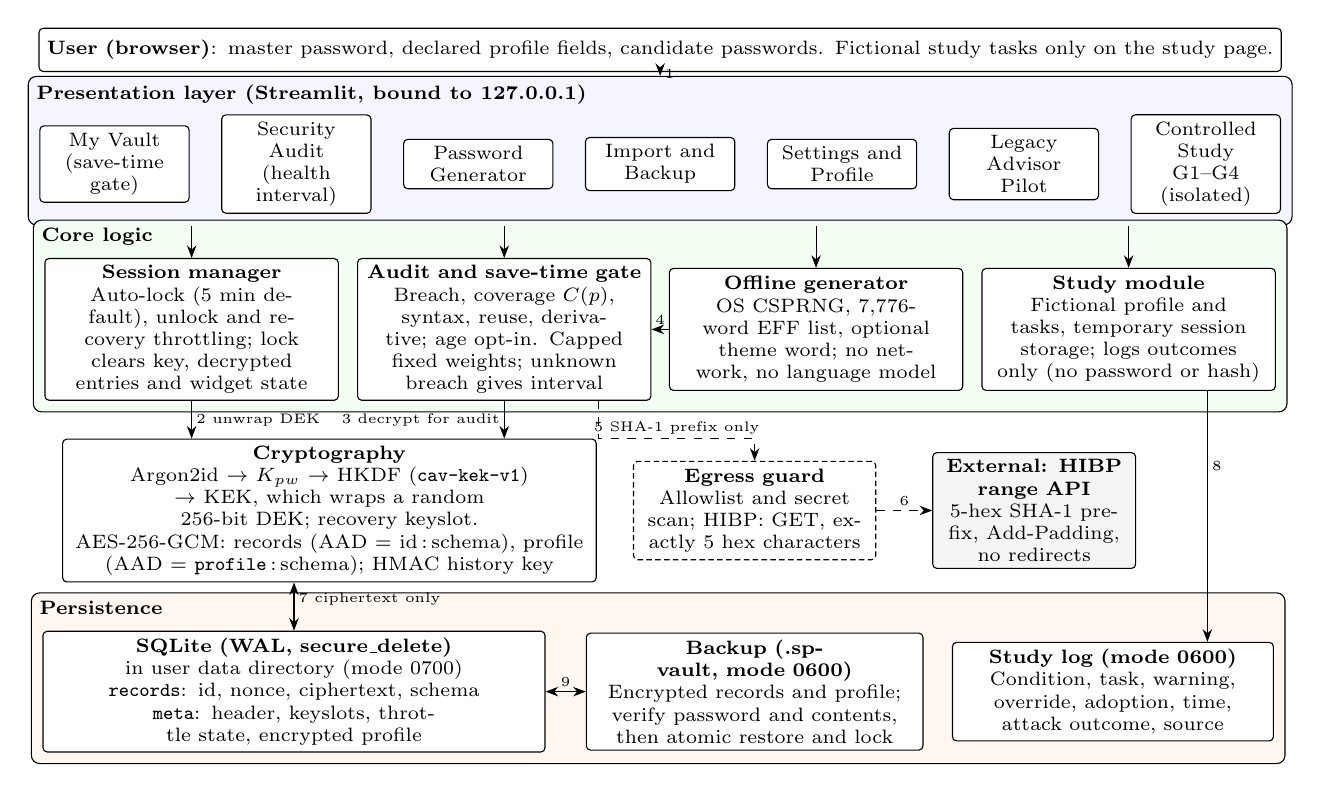
\begin{tikzpicture}[
  font=\scriptsize,
  >={Stealth[length=1.6mm]},
  box/.style={draw, rounded corners=1.5pt, align=center, inner sep=2.5pt, fill=white},
  page/.style={box, text width=1.72cm, minimum height=0.62cm},
  core/.style={box, text width=3.55cm, minimum height=1.55cm},
  layer/.style={draw, rounded corners=3pt, inner sep=4pt},
  lab/.style={font=\scriptsize\bfseries, anchor=north west, inner sep=3pt},
  num/.style={font=\tiny, inner sep=1.5pt}
]
% User
\node[box, text width=15.6cm, minimum height=0.55cm] (user) at (0,0)
  {\textbf{User (browser)}: master password, declared profile fields, candidate passwords. Fictional study tasks only on the study page.};
% Pages
\begin{scope}[yshift=-1.45cm]
\node[page] (p1) at (-6.93,0) {My Vault\\(save-time gate)};
\node[page] (p2) at (-4.62,0) {Security Audit\\(health interval)};
\node[page] (p3) at (-2.31,0) {Password\\Generator};
\node[page] (p4) at (0,0) {Import and\\Backup};
\node[page] (p5) at (2.31,0) {Settings and\\Profile};
\node[page] (p6) at (4.62,0) {Legacy Advisor\\Pilot};
\node[page] (p7) at (6.93,0) {Controlled Study\\G1--G4 (isolated)};
\end{scope}
% Core
\begin{scope}[yshift=-3.55cm]
\node[core] (sess) at (-5.95,0) {\textbf{Session manager}\\Auto-lock (5 min default), unlock and recovery throttling; lock clears key, decrypted entries and widget state};
\node[core] (aud) at (-1.98,0) {\textbf{Audit and save-time gate}\\Breach, coverage $C(p)$, syntax, reuse, derivative; age opt-in. Capped fixed weights; unknown breach gives interval};
\node[core] (gen) at (1.98,0) {\textbf{Offline generator}\\OS CSPRNG, 7,776-word EFF list, optional theme word; no network, no language model};
\node[core] (stu) at (5.95,0) {\textbf{Study module}\\Fictional profile and tasks, temporary session storage; logs outcomes only (no password or hash)};
\end{scope}
% Crypto, egress and external service
\begin{scope}[yshift=-5.85cm]
\node[box, text width=6.6cm, minimum height=1.25cm] (cry) at (-4.2,0) {\textbf{Cryptography}\\Argon2id $\rightarrow$ $K_{pw}$ $\rightarrow$ HKDF (\texttt{cav-kek-v1}) $\rightarrow$ KEK, which wraps a random 256-bit DEK; recovery keyslot.\\AES-256-GCM: records (AAD = id\,:\,schema), profile (AAD = \texttt{profile}\,:\,schema); HMAC history key};
\node[box, text width=2.9cm, minimum height=1.25cm, dash pattern=on 2pt off 1.2pt] (egr) at (1.2,0) {\textbf{Egress guard}\\Allowlist and secret scan; HIBP: GET, exactly 5 hex characters};
\node[box, text width=2.4cm, minimum height=1.25cm, fill=gray!8] (hibp) at (4.75,0) {\textbf{External: HIBP range API}\\5-hex SHA-1 prefix, Add-Padding, no redirects};
\end{scope}
% Persistence
\begin{scope}[yshift=-8.15cm]
\node[box, text width=6.2cm, minimum height=1.15cm] (db) at (-4.65,0) {\textbf{SQLite (WAL, secure\_delete)} in user data directory (mode 0700)\\\texttt{records}: id, nonce, ciphertext, schema\\\texttt{meta}: header, keyslots, throttle state, encrypted profile};
\node[box, text width=4.1cm, minimum height=1.15cm] (bak) at (1.2,0) {\textbf{Backup (.spvault, mode 0600)}\\Encrypted records and profile; verify password and contents, then atomic restore and lock};
\node[box, text width=3.9cm, minimum height=1.15cm] (log) at (5.75,0) {\textbf{Study log (mode 0600)}\\Condition, task, warning, override, adoption, time, attack outcome, source};
\end{scope}
% Layer frames with a title strip above the boxes
\coordinate (presTop) at ($(p7.north)+(0,0.34)$);
\coordinate (coreTop) at ($(sess.north)+(0,0.34)$);
\coordinate (persTop) at ($(db.north)+(0,0.34)$);
\begin{scope}[on background layer]
\node[layer, fill=blue!4, fit=(p1)(p7)(presTop)] (pres) {};
\node[layer, fill=green!5, fit=(sess)(stu)(coreTop)] (corel) {};
\node[layer, fill=orange!6, fit=(db)(log)(persTop)] (pers) {};
\end{scope}
\node[lab] at (pres.north west) {Presentation layer (Streamlit, bound to 127.0.0.1)};
\node[lab] at (corel.north west) {Core logic};
\node[lab] at (pers.north west) {Persistence};
% Flows
\draw[->] (user.south) -- node[num, right]{1} (pres.north);
\draw[->] (sess.north |- pres.south) -- (sess.north);
\draw[->] (aud.north |- pres.south) -- (aud.north);
\draw[->] (gen.north |- pres.south) -- (gen.north);
\draw[->] (stu.north |- pres.south) -- (stu.north);
\draw[->] (sess.south) -- node[num, right]{2 unwrap DEK} (sess.south |- cry.north);
\draw[->] (aud.south) -- node[num, left]{3 decrypt for audit} (aud.south |- cry.north);
\draw[->] (gen.west) -- node[num, above]{4} (aud.east);
\draw[->, dashed] ($(aud.south)+(1.2,0)$) -- ++(0,-0.48) -| node[num, pos=0.25, above]{5 SHA-1 prefix only} (egr.north);
\draw[->, dashed] (egr.east) -- node[num, above]{6} (hibp.west);
\draw[<->] (cry.south -| db.north) -- node[num, right, pos=0.35]{7 ciphertext only} (db.north);
\coordinate (s8) at ($(stu.south)+(1.0,0)$);
\draw[->] (s8) -- node[num, right, pos=0.3]{8} (s8 |- log.north);
\draw[<->] (db.east) -- node[num, above]{9} (bak.west);
\end{tikzpicture}
\caption{CAV architecture. Solid arrows are local data flows and dashed arrows are network flows. The only external destination is the HIBP range endpoint. Numbered flows: (1) user input, (2) key unwrap at unlock, (3) decryption for audit, (4) replacement passphrase, (5, 6) breach range query, (7) ciphertext storage, (8) study outcome logging and (9) backup and restore. Credentials and the personal profile are stored only as ciphertext. The study page uses a fictional profile and temporary session storage and never writes to the vault.}
\label{fig:arch}
\end{figure*}

The system is organized in six layers. The \emph{presentation} layer contains the Streamlit pages and shared helpers, and every vault page checks for an unlocked session. The \emph{session} layer handles auto-lock, unlock throttling and in-memory key handling. The \emph{audit and gate} layer analyses decrypted entries in memory and checks candidate credentials at save time. The \emph{cryptography} layer performs key derivation, key wrapping and record and profile encryption. The \emph{persistence} layer uses SQLite in WAL mode with secure deletion enabled. The \emph{network boundary} is an egress guard that inspects outbound requests.

\section{Cryptographic Design}
\textbf{Key hierarchy.} The master password is processed by Argon2id~\cite{rfc9106} with default parameters $m=64$\,MiB, $t=3$ and $p=4$, producing a 32-byte password key $K_{pw}$. A key-encryption key (KEK) is derived from $K_{pw}$, optionally combined with a device secret, using HKDF-SHA256~\cite{rfc5869} with the context label \texttt{cav-kek-v1}. A random 256-bit data-encryption key (DEK) encrypts every record. The DEK is wrapped under the KEK with AES-256-GCM~\cite{gcm} to form a password keyslot. A separate 256-bit recovery key, shown to the user once in grouped base32 form, wraps the DEK in a recovery keyslot. A history key derived from the DEK with the label \texttt{cav-hist-hmac-v1} produces HMAC-SHA256 digests of previous passwords, so reuse can be detected without storing plaintext history. Changing the master password re-wraps the DEK; records are not re-encrypted.

\textbf{Associated data.} Keyslot wraps are authenticated over the canonical header, excluding the keyslot ciphertexts to avoid circular dependence. Each record is authenticated with its identifier and schema version, so ciphertext cannot be moved between rows without detection.

\textbf{Record and profile encryption.} An entry is serialized as canonical JSON with sorted keys and encrypted with AES-256-GCM under the DEK, using a fresh 96-bit nonce. The records table stores only the identifier, nonce, ciphertext with tag and schema version. The personal profile (first name, surname, city, birth year and theme) is encrypted under the same DEK and bound to the label \texttt{profile} and the schema version. Writing a profile without an unlocked DEK raises an authentication error, so there is no plaintext write path. A legacy plaintext profile is not returned while the vault is locked. It is migrated to ciphertext on the first authenticated read, and a failed migration is reported rather than suppressed. SQLite secure deletion is enabled for future deletions and updates. It does not erase historical copies, snapshots or flash-storage remnants.

\textbf{Backup and restore.} Encrypted backups use a \texttt{.spvault} format that contains the header, the record ciphertexts and the encrypted profile. A backup is refused if the stored profile has not yet been migrated, and backup files are written with mode 0600. Restore first checks the record structure, duplicate identifiers and the declared record count. The application then verifies the backup master password by decrypting every entry and the profile, and only then replaces the stored header, profile and records in one transaction, so records encrypted under different keys are never mixed. A tampered backup leaves the previous vault usable. After a successful restore the session is locked.

\textbf{Unlock throttling.} Failed unlock attempts incur delays of 0, 0, 2, 4 and 8 seconds, doubling thereafter and capped at 300 seconds. The counter and next-allowed time persist across restarts and reset on success. Recovery-key attempts use the same throttle.

\textbf{Master-password policy.} A new or rotated master password must have a zxcvbn score of at least 3, no HIBP hits, and a personal-context coverage below 0.3 when a profile exists. If the HIBP check cannot be completed, creation is not blocked.

\textbf{Session cleanup.} The DEK is held in a mutable buffer that is overwritten on lock or timeout. Locking also deletes decrypted entries, plaintext widget values, pending credential objects, generated values and cached audit reports from the session, keeping only the store handle and the timeout setting. Python cannot guarantee that no copies of immutable strings remain in memory, so this protection is best-effort.

\section{Context-Aware Assessment}
\textbf{Signals and risk.} For each entry $i$, the signals in Table~\ref{tab:signals} are computed. Breach status $b_i$ is 1 if the HIBP count is positive, 0 if it is zero, and \emph{unknown} if the check failed. Coverage $C_i\in[0,1]$ is defined below. Syntactic weakness $s_i$, reuse $r_i$ and derivative membership $d_i$ are binary. Reuse is computed by excluding the current entry by its identifier rather than its site name, so two accounts at the same service that share a password count as reuse. Age $a_i$ is $\min(1,\text{days}/365)$ for entries older than the rotation-policy period (90 days by default) and 0 otherwise. Its weight $w_a$ is 0 unless a policy or research configuration enables it. Age is shown as descriptive information and is not treated as evidence of compromise, consistent with current NIST guidance against routine periodic changes~\cite{nist63b4}.

\begin{table}[t]
\caption{Assessment Signals and Default Weights}
\label{tab:signals}
\centering\footnotesize
\begin{tabular}{@{}l c >{\raggedright\arraybackslash}p{3.55cm} c@{}}
\toprule
Signal & Sym. & Definition & Weight\\
\midrule
Breach & $b_i$ & 1 if HIBP count $>0$; unknown if the check fails & 0.45\\
Coverage & $C_i$ & Personal-context coverage in $[0,1]$; flagged at $\geq 0.3$ & 0.25$^{*}$\\
Syntax & $s_i$ & 1 if zxcvbn score $<3$ & 0.15\\
Reuse & $r_i$ & 1 if another entry has the same password & 0.10$^{*}$\\
Derivative & $d_i$ & 1 if in a derivative family & 0.05$^{*}$\\
Age & $a_i$ & $\min(1,\text{days}/365)$ beyond the rotation period & 0 (opt-in)\\
\bottomrule
\multicolumn{4}{@{}p{\columnwidth}@{}}{\scriptsize $^{*}$Coverage, reuse and derivative contributions share a cap of 0.35. The submitted baseline used 0.40/0.25/0.15/0.10/0.05/0.05 without a cap (B6).}
\end{tabular}
\end{table}

The per-entry risk is
\begin{align}
R_i=\min\!\Big(1,\;&0.45\,b_i+0.15\,s_i+w_a a_i\nonumber\\
&+\min\big(0.35,\;0.25\,C_i+0.10\,r_i+0.05\,d_i\big)\Big).
\label{eq:risk}
\end{align}
The 0.35 cap limits how much correlated personal, reuse and derivative evidence can add. It is a heuristic, not a calibrated correction for correlation. With $w_a=0$ and no breach evidence, $R_i$ cannot exceed $0.15+0.35=0.50$. The score is a priority, not a probability of compromise. A fitted model can be loaded only when explicitly configured, and its coefficients are validated as finite and limited to known features. No model file is loaded implicitly.

Each account has a criticality $w_i\in\{1,2,3\}$, and the Vault Health Score is
\begin{equation}
\mathrm{VHS}=100\times\left(1-\frac{\sum_i w_i R_i}{\sum_i w_i}\right).
\label{eq:vhs}
\end{equation}
An empty vault scores 100. Scores map to grades A ($\geq 85$), B ($\geq 70$), C ($\geq 50$) and F (otherwise).

\textbf{Unknown breach status.} When a breach check fails, no value is substituted for $b_i$. The entry is scored at both endpoints, $R_i^{-}=R_i|_{b_i=0}$ and $R_i^{+}=R_i|_{b_i=1}$, and the corresponding sums in (\ref{eq:vhs}) give a health interval $[\mathrm{VHS}^{-},\mathrm{VHS}^{+}]$. The Security Audit page reports the interval, marks the assessment incomplete and replaces the letter grade. The interval covers missing breach evidence only, not other uncertainty in the heuristic.

\textbf{Personal-context coverage.} Let $p$ be the candidate password and $N(p)$ its normalized form: lowercased, with whitespace and the separators \texttt{- \_ . : ; , | / \textbackslash} removed, and with the reverse leetspeak map 0$\to$o, 1$\to$i, 2$\to$z, 3$\to$e, 4$\to$a, 5$\to$s, 7$\to$t, 8$\to$b, @$\to$a, \$$\to$s, !$\to$i and +$\to$t applied. The first name, surname and city are normalized in the same way and used if they have at least three characters. Each attribute contributes its full form, its four-character prefix if it has at least five characters, and its three-character prefix if it has at least four characters. Prefixes that are common short English words are skipped. For each attribute, the longest token found in $N(p)$ is kept, and $U(p)$ is the set of positions of $N(p)$ covered by occurrences of the kept tokens. The birth year contributes $Y(p)=4$ characters if the four-digit year occurs. Otherwise it contributes 2 if the two-digit form occurs and either another attribute was matched or a boundary rule for trailing digits is satisfied. A detected name therefore no longer causes an absent two-digit year to be reported. The coverage is
\begin{equation}
C(p)=\min\!\left(1,\;\frac{|U(p)|+Y(p)}{|p|}\right).
\label{eq:cov}
\end{equation}
A password is flagged in the audit when $C(p)\geq 0.3$. The matched fields, including a \emph{multi-attribute} flag when two matched tokens appear adjacent in either order, are returned so that the warning can name the exposure.

\textbf{Derivative families.} Each password is reduced to a base by lowercasing it, stripping leading and trailing digits and punctuation, applying the reverse leet map and stripping again. Two entries are related when their bases are identical (length at least 3), when their base similarity is at least 85 on the rapidfuzz ratio scale (bases of at least four characters), or when the raw Levenshtein distance is at most 2 for passwords of at least six characters. In \emph{chain} mode, Union-Find with iterative path halving forms connected components. A component can therefore contain two passwords that do not satisfy the pair rule directly. In \emph{pairwise} mode, entries sorted by identifier are grouped greedily so that every pair in a group satisfies the rule. This is a deterministic complete-link grouping, not a maximum-clique search. Pairs are compared in a streaming loop without an $n\times n$ matrix, but the worst-case number of comparisons remains quadratic. The save-time gate and the audit use the same pair rule.

\textbf{Breach check.} The SHA-1 digest is computed locally, and only its first five hexadecimal characters are sent to the Pwned Passwords range endpoint~\cite{hibp} with the Add-Padding header. The egress guard validates the endpoint and method before sending, and redirects are disabled. A response must have status 200, and every line must contain a 35-character hexadecimal suffix and a count. A failed, empty or malformed response produces an unknown status, never a clean one. Network errors are retried once.

\section{Save-Time Intervention}
\textbf{Save-time gate.} When a user adds or edits an entry, the candidate is checked for breach status, personal context, structural strength, exact reuse and derivative relationships before it is written. In the gate, any matched profile field produces a warning even when the coverage is below 0.3. If any finding fires, the user sees the reasons and three actions: use the generated passphrase, edit the candidate or save anyway. An unavailable breach check produces an explicit warning that the password could not be verified. Saving remains possible with that warning, so an outage does not block the user. Editing an entry preserves its creation date and password history and records the modification time, and vault changes invalidate any cached audit report.

\textbf{Offline generator.} Suggestions use no network service and no language model. Passphrases draw words uniformly from the 7,776-word EFF large wordlist~\cite{eff} using the operating system's CSPRNG. Each word contributes $\log_2 7776\approx 12.9$ bits. The gate's suggestion uses four capitalized words with a digit and a symbol, and an optional theme word from the profile. The interface reports generation entropy computed from pool sizes and states that it is not a guarantee against compromise. Earlier wording such as ``un-crackable'' and ``zero reuse risk'' was removed. Random passwords include at least one character from each enabled class.

\textbf{Controlled study interface.} An isolated page implements four conditions with the same fictional profile, the same fictional previous password and the same contextual rules: \textbf{G1} receives structural feedback only; \textbf{G2} receives contextual feedback after the credential is saved to temporary study storage, with the warning kept until the participant edits or keeps it; \textbf{G3} receives the same feedback before saving; and \textbf{G4} additionally receives a locally generated alternative. Each participant completes three tasks (a shop, an email service and a social account). Consent is required before any task starts. Human collection is refused unless an ethics reference and an allocation seed are configured, and every record is labelled as demo, synthetic or human. Allocation is a seeded hash of the participant identifier. This is reproducible but not guaranteed to be balanced. The log stores the condition, task, warning, override, adoption, total decision time and an independent outcome: whether the final fictional password is recovered by the S5 attacker within 1,000 guesses. No password or password hash is stored. The analysis script reports participant-level estimates with clustered bootstrap intervals and the contrasts G3$-$G2, G4$-$G3 and G4$-$G1. It rejects duplicate participant-task records, inconsistent assignments and logs without provenance. The earlier loss-framed versus neutral Advisor Pilot page is retained as a legacy page.

\section{Implementation}
\label{sec:impl}
CAV uses Streamlit, argon2-cffi, the cryptography library, zxcvbn-python, requests, rapidfuzz, platformdirs and pyperclip. The research scripts also use NumPy and scikit-learn. Tested versions are pinned in a lock file. The vault is stored in the operating system's user-data directory with mode 0700 on POSIX systems. Clipboard contents are cleared after 20 seconds, but only if the clipboard still holds the copied secret. Auto-lock defaults to five minutes and can be set from 1 to 60 minutes. Import supports Chrome and Bitwarden CSV exports and generic column layouts. A plaintext CSV export also exists, with a disclosure warning. The Settings page shows the deployed weights read-only. Earlier sliders that appeared to change the weights but were never applied were removed.

All outbound requests pass through the egress guard. Its allowlist accepts the HIBP range endpoint with exactly five hexadecimal characters and localhost. It also retains a pattern for the chat endpoint used by the earlier advisor, but no code path now calls it. URLs, request bodies and non-authorization headers are scanned for active secret strings, and any violation raises an error.

The automated suite contains 102 tests, and all passed on 10 November 2026 (Python 3.14.7, macOS 27.3, Apple M5, 16\,GB RAM), with one deprecation warning from zxcvbn-python. The suite covers cryptographic round trips, nonce uniqueness, associated-data swaps, recovery keys and a scan for plaintext in stored bytes. It also covers keyless profile writes, legacy profile migration, backup profile preservation, atomic rejection of tampered restores, unknown breach intervals, malformed HIBP responses, session cleanup, same-service reuse and absent birth-year matches. Streamlit AppTest exercises all four study conditions and the vault's warn-before-save and override behaviour. HIBP and the clipboard are replaced by deterministic fixtures, so the tests check the application's contract, not live services.

\section{Evaluation Method}
\textbf{Data.} The evaluation uses a synthetic fixture of 11,022 examples from 1,002 fictional profiles (seed 42). Each profile contributes one example in each of 11 categories: direct, leetspeak, partial, reordered, multi-attribute, history-derived, exact reuse, unrelated weak, random, hard negative and unseen transformation. Profiles are assigned to training, validation and test partitions (334 profiles each; 3,674 held-out examples). A validator rejects any profile, family, template or exact password that appears in more than one partition. Separators differ by partition. The personal label (E1) is a construction label. Attack outcomes (E2 and E3) are measured separately by running an attacker and are never inferred from detector warnings. In this fixture, breach evidence is a small blocklist assigned to the unrelated-weak category, not a live HIBP result. The generator was written by the authors. It is therefore an engineering fixture for reproducible testing, not independent validation data.

\textbf{Attacker.} A deterministic bounded attacker produces distinct, ordered guesses without seeing the target. S1 uses eight common words with fixed suffixes and appended numbers. S2 joins pairs of declared attributes with separators and appends numbers to each attribute. S3 mutates the previous password: it shifts four-digit years by $\pm 1$ or $\pm 2$, appends suffixes and replaces trailing digits and symbols with numbers. S4 interleaves S2 and S3, and S5 interleaves all three. Budgets of 100 and 1,000 guesses were executed, and the first matching rank and the actual number of distinct guesses were recorded.

\textbf{Baselines and protocol.} All methods are scored against the same S5 outcome at 1,000 guesses (E2). B1 is the binary zxcvbn weakness flag, B2 the breach fixture, B3 their maximum, B4 personal coverage, B5 reuse or derivative membership, and B6 the submitted six-signal weights without the cap. CAV denotes the current score in (\ref{eq:risk}), and B7 is a logistic regression fitted on the training partition only. Each threshold is selected on the validation partition as the one with the highest recall at a false-positive rate (FPR) of at most 5\%, and it is then frozen for the test partition. Each of the six signals is ablated twice: by zeroing it under the fixed B6 weights without renormalization, and by refitting the logistic model without it. A profile-level paired bootstrap with 300 replicates gives 95\% intervals for recall differences against B1. A faithful published contextual model (B8) was not reproduced.

\section{Results}
\textbf{E1: personal-context detection.} Table~\ref{tab:e1} reports the coverage score $C(p)$ on held-out data at the validation-selected threshold of 0.25. The production flag uses 0.3. Recall was 1.000 for the direct, leetspeak, partial, reordered, multi-attribute, history-derived and exact-reuse categories (334 each). History-derived and exact-reuse examples contain the first name, which is why the coverage score flags them. The detector recovered only 5 of 334 unseen transformations (recall 0.015). This is the main source of false negatives, and it shows that the detector recognises the transformation families it was designed for. It flagged 25 of 334 hard negatives (FPR 0.075), 1 of 334 unrelated weak passwords and none of the random strings.

\begin{table}[t]
\caption{E1 Held-Out Personal-Context Detection ($n=3{,}674$)}
\label{tab:e1}
\centering\footnotesize
\begin{tabular}{@{}lc@{\hspace{14pt}}lc@{}}
\toprule
Metric & Value & Metric & Value\\
\midrule
Precision & 0.989 & FPR & 0.026\\
Recall & 0.877 & Balanced accuracy & 0.925\\
F1 & 0.930 & PR-AUC (AP) & 0.966\\
TP / FP & 2,343 / 26 & ROC-AUC & 0.918\\
TN / FN & 976 / 329 & Brier score & 0.154\\
\bottomrule
\end{tabular}
\end{table}

\textbf{E2: matched baselines.} Of the 3,674 held-out examples, 2,183 (59.4\%) were recovered by S5 within 1,000 guesses. Table~\ref{tab:e2} lists the results. The binary syntax flag selected no positives at the validation constraint. This reflects that operating point, not evidence that zxcvbn is ineffective. Both CAV and B6 reached the same recall as the breach fixture alone (0.153). Without breach evidence the current score cannot exceed 0.50, below its selected threshold of 0.60, so it flagged only breach-fixture items. Its PR-AUC of 0.781 shows that its ranking carries information that a single fixed threshold does not use. The logistic baseline reached a recall of 0.503 at an FPR of 0.048. The bootstrap interval for the recall difference against B1 was [0.152, 0.154] for CAV and [0.497, 0.508] for B7. These intervals are narrow because the fixture uses a small set of deterministic templates.

\begin{table}[t]
\caption{E2 Held-Out Results Against S5 at 1,000 Guesses}
\label{tab:e2}
\centering\footnotesize
\begin{tabular}{@{}lccccc@{}}
\toprule
Method & Prec. & Recall & FPR & PR-AUC & Brier\\
\midrule
B1 syntax flag & -- & 0.000 & 0.000 & 0.580 & 0.594\\
B2 breach fixture & 1.000 & 0.153 & 0.000 & 0.656 & 0.503\\
B3 syntax or breach & -- & 0.000 & 0.000 & 0.580 & 0.594\\
B4 personal coverage & -- & 0.000 & 0.000 & 0.764 & 0.236\\
B5 reuse/derivative & 1.000 & 0.306 & 0.000 & 0.718 & 0.412\\
B6 submitted weights & 1.000 & 0.153 & 0.000 & 0.773 & 0.319\\
CAV (current) & 1.000 & 0.153 & 0.000 & 0.781 & 0.333\\
B7 logistic & 0.938 & 0.503 & 0.048 & 0.956 & 0.044\\
\bottomrule
\multicolumn{6}{@{}p{\columnwidth}@{}}{\scriptsize Thresholds selected on validation at FPR $\leq$ 5\%. ``--'': no positive predictions. PR-AUC is average precision.}
\end{tabular}
\end{table}

\textbf{Ablation and calibration.} Table~\ref{tab:abl} reports the ablations. Under fixed weights, removing breach evidence reduced recall to 0, and removing the syntax signal increased PR-AUC from 0.773 to 0.903. In the refitted models, removing breach or derivative evidence reduced recall from 0.503 to 0.350. The fitted syntax coefficient was negative ($-4.20$), so weak structure was associated with lower recovery in this fixture. We attribute this to the fixture's construction and do not generalise it. Calibration bands confirm that the fixed score is not a probability. For CAV, examples scored in $[0,0.2)$ (mean score 0.055, $n=1{,}336$) were recovered 25.0\% of the time, and those in $[0.2,0.4)$ (mean 0.250, $n=2{,}004$) 75.6\% of the time. Scores of 0.4 and above ($n=334$) were all recovered. The logistic model is promising on this fixture, but it is neither externally validated nor deployed. The fitted coefficients are exported as research-only data.

\begin{table}[t]
\caption{E2 Signal Ablations (Held-Out Recall / PR-AUC)}
\label{tab:abl}
\centering\footnotesize
\begin{tabular}{@{}lcc@{}}
\toprule
Removed signal & Fixed B6 weights & Refitted logistic\\
\midrule
None (full model) & 0.153 / 0.773 & 0.503 / 0.956\\
Breach & 0.000 / 0.670 & 0.350 / 0.851\\
Coverage & 0.153 / 0.707 & 0.459 / 0.835\\
Syntax & 0.232 / 0.903 & 0.503 / 0.956\\
Reuse & 0.153 / 0.767 & 0.503 / 0.956\\
Derivative & 0.153 / 0.766 & 0.350 / 0.935\\
Age & 0.153 / 0.781 & 0.459 / 0.956\\
\bottomrule
\end{tabular}
\end{table}

\textbf{E3: attacker scenarios.} Table~\ref{tab:e3} reports the recovery rate for each scenario and the held-out recall of CAV and B7 at their frozen S5 thresholds. Combining sources increased recovery. At 1,000 guesses S5 recovered 59.4\% of examples, against 32.1\% for personal information alone and 18.2\% for history alone. CAV detected all S1 recoveries but none of the S2, S3 or S4 recoveries, because personal and history evidence alone cannot reach its threshold. Because the thresholds were selected for S5, the FPRs for the other scenarios are not constrained. For example, CAV's FPR under S2 was 0.134. Non-recovery means only that this attacker did not guess the password within the budget. It does not establish that the password is safe.

\begin{table}[t]
\caption{E3 Recovery by Scenario and Held-Out Recall ($n=3{,}674$)}
\label{tab:e3}
\centering\footnotesize
\begin{tabular}{@{}lccccc@{}}
\toprule
& \multicolumn{2}{c}{Recovered (\%)} & \multicolumn{3}{c}{Recall at 100 / 1,000}\\
\cmidrule(lr){2-3}\cmidrule(l){4-6}
Scenario & 100 & 1,000 & B1 & CAV & B7\\
\midrule
S1 general & 9.1 & 9.1 & 0 / 0 & 1.000 / 1.000 & 1.000 / 1.000\\
S2 personal & 32.1 & 32.1 & 0 / 0 & 0.000 / 0.000 & 0.080 / 0.080\\
S3 history & 18.2 & 18.2 & 0 / 0 & 0.000 / 0.000 & 1.000 / 1.000\\
S4 S2+S3 & 41.2 & 50.3 & 0 / 0 & 0.000 / 0.000 & 0.504 / 0.413\\
S5 all & 50.3 & 59.4 & 0 / 0 & 0.181 / 0.153 & 0.593 / 0.503\\
\bottomrule
\end{tabular}
\end{table}

\textbf{Derivative clustering.} A separate fixture planted 30 families of three year variants (2023, 2024, 2025) of a random 12-letter base, together with 30 unrelated random strings (120 entries, 7,140 pairs, 90 within-family pairs). Both chain and pairwise modes recovered every family pair with no false pairs (pairwise precision and recall 1.0, adjusted Rand index 1.0, B-cubed precision and recall 1.0). The S3 history attacker guessed all 90 within-family pairs within 1,000 guesses. This tests one narrow transformation and should not be generalised.

\textbf{E5: security validation.} Table~\ref{tab:sec} summarizes the security matrix. Each property was exercised by passing tests on fictional data and temporary databases. The table records what the tests do not cover.

\begin{table}[t]
\caption{E5 Security Matrix: Tested Property and Remaining Limit}
\label{tab:sec}
\centering\scriptsize
\begin{tabular}{@{}p{2.9cm}p{5.2cm}@{}}
\toprule
Tested property (pass) & Remaining limitation\\
\midrule
No plaintext credential or profile tokens in database or backup bytes & Ciphertext lengths, record counts and identifiers are visible; old files are not erased\\
Modified ciphertext, tag or record ID fails to decrypt & Deletion or replay of a whole earlier vault is not prevented\\
Argon2id timings reported (Table~\ref{tab:perf}) & Not adversary throughput or a cost guarantee\\
Wrong recovery keys rejected; recovery throttled & Recovery key is reusable until revoked\\
Keyless profile writes rejected; migration encrypts & Secure deletion cannot erase snapshots or remnants\\
HIBP request: GET, 5-hex prefix, padding, no redirects & No packet capture or traffic-correlation analysis\\
Clipboard cleared only if unchanged (simulated) & No OS clipboard-history or sync inspection\\
Network error or malformed body gives unknown & Bounds cover breach uncertainty only\\
Lock clears key, decrypted entries and widget state & Immutable Python copies and rendered secrets\\
Restore verifies password and contents, then atomic & No authenticated whole-file manifest\\
\bottomrule
\end{tabular}
\end{table}

\textbf{E6: local performance.} Table~\ref{tab:perf} reports medians of three timed trials on random fictional vaults on the host described in Section~\ref{sec:impl}. Syntax and coverage computation were real, and HIBP was stubbed, so network latency is excluded. Full audit time grew from 6\,ms at 10 entries to 8.5\,s at 5,000 entries. At 5,000 entries derivative grouping alone took 4.7\,s, and removing it reduced the audit to 2.8\,s, which is consistent with quadratic pair comparison. Removing the zxcvbn computation reduced it to 4.9\,s. The save-time gate stayed below 7\,ms at every size. Peak traced Python allocation for the full audit was 17.1\,MiB at 5,000 entries. This excludes native allocations. The default Argon2id setting took 37.8\,ms, well below the 300--600\,ms target in the development plan, so the margin against offline guessing of the master password is smaller than planned.

\begin{table}[t]
\caption{E6 Median Local Latency (ms) and Argon2id Timing}
\label{tab:perf}
\centering\footnotesize
\begin{tabular}{@{}rrrrr@{}}
\toprule
Entries & Full audit & Save gate & Derivative & Audit w/o deriv.\\
\midrule
10 & 5.98 & 1.32 & 0.03 & 5.41\\
100 & 52.72 & 1.25 & 1.79 & 49.48\\
500 & 284.88 & 1.87 & 43.44 & 244.29\\
1,000 & 685.80 & 2.48 & 183.27 & 505.24\\
5,000 & 8,508.28 & 6.84 & 4,736.90 & 2,760.66\\
\midrule
\multicolumn{4}{@{}l}{Argon2id ($m$, $t$, $p$)} & Time\\
\midrule
\multicolumn{4}{@{}l}{32\,MiB, 2, 2} & 16.68\\
\multicolumn{4}{@{}l}{64\,MiB, 2, 4} & 25.39\\
\multicolumn{4}{@{}l}{64\,MiB, 3, 4 (default)} & 37.84\\
\multicolumn{4}{@{}l}{64\,MiB, 4, 4} & 49.29\\
\multicolumn{4}{@{}l}{128\,MiB, 2, 4} & 50.59\\
\bottomrule
\end{tabular}
\end{table}

\textbf{Human-subject evidence.} No human-subject results are reported. No participants were recruited for the four-condition study. An earlier 10-participant comparison of loss-framed and neutral warnings is not reported, because its records and assignment procedure could not be verified.

\section{Discussion and Limitations}
Keeping the signals separate lets a warning name the specific exposure and avoids a single rejection threshold, which earlier work found to cause very high rejection rates~\cite{saintjean}. The synthetic results show both what this design does and what it misses. Personal-context detection works for the transformation families it encodes, but not for unseen ones. Vault relationships carry attack-relevant information: B5 alone recalled 0.306, and removing derivative evidence lowered the refitted recall. The current fixed weights, however, use little of that information at a strict false-positive limit. We state the following limitations explicitly.
\begin{enumerate}
\item \textbf{Data.} The fixture and its labels were produced by the authors' own generator, with broad templates that are related across partitions. No independent, adjudicated or multilingual dataset was used, and per-category confidence intervals were not computed.
\item \textbf{Attacks and baselines.} The attacker is a simple deterministic generator, not MDIGuess~\cite{mdiguess} or the attack of Ou et al.~\cite{ou2026}. Budgets of $10^4$ and $10^5$ were not run, and no published contextual model (B8) was reproduced. No superiority claim is made.
\item \textbf{Scoring.} The weights and the 0.35 cap are heuristics. The logistic baseline was fitted and tested on the same synthetic distribution and is not deployed. Chain clustering can link passwords transitively, and its worst-case cost is quadratic.
\item \textbf{Breach evidence.} Score intervals cover missing breach evidence only. The gate and master-password creation still allow saving when HIBP is unreachable, with a warning in the gate.
\item \textbf{Storage and backup.} Ciphertext lengths, counts and identifiers are visible. Rollback or deletion of a whole vault, and record deletion with an adjusted unauthenticated count in a backup, are not detected. Legacy backups without a profile cannot restore it. Historical plaintext artifacts may persist outside SQLite's control.
\item \textbf{Host and memory.} Memory clearing is best-effort in Python. The clipboard and network tests use stubs, and no packet capture was performed. The Argon2id setting is below the planned timing target.
\item \textbf{Behaviour.} The study interface has not been used with participants. A definitive study needs ethics approval, a power analysis, a randomized and counterbalanced allocation (task order is currently fixed), questionnaires on understanding and usability, delayed recall and follow-up. Retained study credentials are temporary and are not real account changes.
\item \textbf{Performance.} The measurements come from one host with three repeats, so the tail quantiles are descriptive. Network latency and native memory were not measured.
\end{enumerate}

\section{Conclusion and Future Work}
CAV shows that a local password manager can assess breach evidence, declared personal context, structure, reuse and derivative relationships while keeping credentials and personal attributes encrypted on disk and off the network. It reports missing breach evidence as an interval instead of guessing a value, and it can intervene before a risky credential is stored. The revised implementation is covered by 102 passing tests and a reproducible synthetic evaluation. That evaluation is useful for debugging rather than as confirmation. The detector misses unseen transformations, and the current fixed weights recover few attack-recoverable passwords at a strict false-positive limit, while a fitted model on the same features does better on this fixture. Claims are limited to the implemented mechanisms and these synthetic measurements.

Future work includes an independent, adjudicated benchmark with per-category uncertainty; a faithful reproduction of published targeted-guessing models at larger budgets; validated calibration before any fitted model is deployed; an ethics-approved, adequately powered and counterbalanced study of G1--G4; an authenticated backup manifest; dictionary-word checks in the gate; queued breach re-checks; measurements on more hardware with real network latency; post-login keystroke verification~\cite{parkinson,rusli}; and passwordless authentication with FIDO2/WebAuthn.

\begin{thebibliography}{99}
\bibitem{jubur} M. Jubur, P. Shrestha, and N. Saxena, ``An in-depth analysis of password managers and two-factor authentication tools,'' \emph{ACM Comput. Surv.}, vol.~57, no.~5, Art. no.~128, 2025, doi: 10.1145/3711117.
\bibitem{aiswarya} R. Aiswarya, J. Raveendran, and V. Banahatti, ``Behavioral attributes in password reuse: Analysis of password practices in work and personal spaces,'' in \emph{Proc. 13th Indian Conf. Human-Computer Interaction (IndiaHCI)}, 2022, doi: 10.1145/3570211.3570212.
\bibitem{farcasin} M. Farcasin, A. Guli, and E. Chan-Tin, ``Fluid passwords: Mitigating the effects of password leaks at the user level,'' arXiv:1708.09333, 2017.
\bibitem{atzori2024} M. Atzori, E. Cal\`o, L. Caruccio, S. Cirillo, G. Polese, and G. Solimando, ``Evaluating password strength based on information spread on social networks: A combined approach relying on data reconstruction and generative models,'' \emph{Online Soc. Netw. Media}, vol.~42, Art. no.~100278, 2024, doi: 10.1016/j.osnem.2024.100278.
\bibitem{he} D. He, Z. Liu, S. Chan, B. Zhou, and M. Guizani, ``Evaluating the impact of special characters on password security: A comparative analysis,'' \emph{IEEE Netw.}, Nov./Dec. 2025.
\bibitem{umejiaku2023} A. P. Umejiaku, P. Dhakal, and V. S. Sheng, ``Balancing password security and user convenience: Exploring the potential of prompt models for password generation,'' \emph{Electronics}, vol.~12, no.~10, Art. no.~2159, 2023, doi: 10.3390/electronics12102159.
\bibitem{nebbione} G. Nebbione and M. C. Calzarossa, ``A methodological framework for AI-assisted security assessments of Active Directory environments,'' \emph{IEEE Access}, vol.~11, pp.~15119--15130, 2023, doi: 10.1109/ACCESS.2023.3244490.
\bibitem{ou2026} W. Ou, C. Sun, M. Pang, Q. Yue, Y. Zhang, and W. Han, ``Improving targeted password guessing attacks by using personally identifiable information and old password,'' \emph{Cybersecurity}, vol.~9, no.~1, Art. no.~9, 2026, doi: 10.1186/s42400-025-00430-0.
\bibitem{mdiguess} X. Tang, W. Peng, Q. Wu, Z. Wei, T. Zhao, and S. Chen, ``MDIGuess: Improving targeted password guessing by combining multi-dimensional heterogeneous information,'' \emph{IEEE Trans. Inf. Forensics Security}, vol.~21, pp.~7423--7438, 2026, doi: 10.1109/TIFS.2026.3723136.
\bibitem{wheeler} D. L. Wheeler, ``zxcvbn: Low-budget password strength estimation,'' in \emph{Proc. 25th USENIX Security Symp.}, 2016, pp.~157--173.
\bibitem{saintjean} D. Saint-Jean, B. Al Smadi, and C. Sumlin, ``A breach-adjusted entropy model for password strength evaluation,'' in \emph{Proc. Int. Conf. Artificial Intelligence, Computer, Data Sciences and Applications (ACDSA)}, Boracay Island, Philippines, Feb. 2026, doi: 10.1109/ACDSA67686.2026.11467996.
\bibitem{alatawi} M. N. Alatawi, ``Cipher-Guard: A machine learning model for adaptive and context-aware password security,'' \emph{IET Inf. Secur.}, vol.~2026, Art. no.~3930060, 2026, doi: 10.1049/ise2/3930060.
\bibitem{weir} M. Weir, S. Aggarwal, B. de Medeiros, and B. Glodek, ``Password cracking using probabilistic context-free grammars,'' in \emph{Proc. IEEE Symp. Security and Privacy}, 2009, pp.~391--405.
\bibitem{nist63b4} D. Temoshok \emph{et al.}, ``Digital identity guidelines: Authentication and authenticator management,'' NIST Special Publication 800-63B-4, Jul. 2025, doi: 10.6028/NIST.SP.800-63B-4.
\bibitem{nosenko} A. Nosenko, Y. Cheng, and H. Chen, ``Password and passphrase guessing with recurrent neural networks,'' \emph{Inf. Syst. Frontiers}, vol.~25, no.~2, pp.~549--565, 2023, doi: 10.1007/s10796-022-10325-x.
\bibitem{sun} Y. Sun, ``A password algorithm recognition and classification framework based on BiGRU attention network,'' \emph{J. Comput. Virol. Hacking Tech.}, vol.~22, Art. no.~41, 2026, doi: 10.1007/s11416-026-00619-y.
\bibitem{xu} M. Xu, W. Han, J. Yu, J. Liu, X. Zhang, Y. Lin, and J. S. Dong, ``On the account security risks posed by password strength meters,'' in \emph{Proc. ACM Asia Conf. Computer and Communications Security (ASIA CCS '25)}, 2025, pp.~1582--1599, doi: 10.1145/3708821.3736202.
\bibitem{atzori2025} M. Atzori, E. Cal\`o, L. Caruccio, S. Cirillo, G. Polese, and G. Solimando, ``Password strength analysis through social network data exposure: A combined approach relying on data reconstruction and generative models,'' arXiv:2511.16716, 2025.
\bibitem{guven} E. Y. G\"uven, A. Boyac\i, and M. A. Ayd\i n, ``A novel password policy focusing on altering user password selection habits: A statistical analysis on breached data,'' \emph{Comput. Secur.}, vol.~113, Art. no.~102560, 2022, doi: 10.1016/j.cose.2021.102560.
\bibitem{dani} J. Dani, B. McCulloh, and N. Saxena, ``When AI defeats password deception! A deep learning framework to distinguish passwords and honeywords,'' arXiv:2407.16964, 2024.
\bibitem{umejiaku2025} A. P. Umejiaku, M. Sonde, and V. S. Sheng, ``Enhancing password security with honeywords and LLMs,'' \emph{J. Inf. Secur. Appl.}, vol.~93, Art. no.~104129, 2025, doi: 10.1016/j.jisa.2025.104129.
\bibitem{kagnici} O. Kagnici, H. Bisgin, and S. Uludag, ``A comparative study of large language models for human-like password generation and predictability,'' in \emph{Proc. 9th Cyber Security in Networking Conf. (CSNet)}, 2025, doi: 10.1109/CSNet67572.2025.11288226.
\bibitem{sai} S. Sai, U. Yashvardhan, V. Chamola, and B. Sikdar, ``Generative AI for cyber security: Analyzing the potential of ChatGPT, DALL-E, and other models for enhancing the security space,'' \emph{IEEE Access}, vol.~12, pp.~53497--53516, 2024, doi: 10.1109/ACCESS.2024.3385107.
\bibitem{arciulo} L. Arciulo and F. Di Nocera, ``The nudging paradigm in cybersecurity research: A PRISMA-based systematic review,'' \emph{Information}, vol.~17, no.~3, Art. no.~264, 2026, doi: 10.3390/info17030264.
\bibitem{zou} Y. Zou, K. Le, P. Mayer, A. Acquisti, A. J. Aviv, and F. Schaub, ``Encouraging users to change breached passwords using the Protection Motivation Theory,'' \emph{ACM Trans. Comput.-Hum. Interact.}, vol.~31, no.~5, Art. no.~63, 2024, doi: 10.1145/3689432.
\bibitem{peer} E. Peer, S. Egelman, M. Harbach, N. Malkin, A. Mathur, and A. Frik, ``Nudge me right: Personalizing online security nudges to people's decision-making styles,'' \emph{Comput. Human Behav.}, vol.~109, Art. no.~106347, 2020, doi: 10.1016/j.chb.2020.106347.
\bibitem{wise} J. Wise and Md. Hoque, ``Lyric-based passwords: Enhancing security and recall with AI,'' \emph{Cyber Security and Applications}, vol.~3, Art. no.~100108, 2025, doi: 10.1016/j.csa.2025.100108.
\bibitem{rfc9106} A. Biryukov, D. Dinu, D. Khovratovich, and S. Josefsson, ``Argon2 memory-hard function for password hashing and proof-of-work applications,'' RFC 9106, Sep. 2021.
\bibitem{rfc5869} H. Krawczyk and P. Eronen, ``HMAC-based extract-and-expand key derivation function (HKDF),'' RFC 5869, May 2010.
\bibitem{gcm} M. Dworkin, ``Recommendation for block cipher modes of operation: Galois/Counter Mode (GCM) and GMAC,'' NIST Special Publication 800-38D, 2007.
\bibitem{hibp} T. Hunt, ``Pwned Passwords: k-anonymity range API,'' Have I Been Pwned. [Online]. Available: \url{https://haveibeenpwned.com/API/v3#PwnedPasswords}
\bibitem{eff} Electronic Frontier Foundation, ``EFF's new wordlists for random passphrases,'' 2016. [Online]. Available: \url{https://www.eff.org/deeplinks/2016/07/new-wordlists-random-passphrases}
\bibitem{parkinson} S. Parkinson, S. Khan, A.-M. Badea, A. Crampton, N. Liu, and Q. Xu, ``An empirical analysis of keystroke dynamics in passwords: A longitudinal study,'' \emph{IET Biometrics}, vol.~12, no.~1, pp.~25--37, 2023, doi: 10.1049/bme2.12087.
\bibitem{rusli} M. E. Rusli and M. N. A. Hasan, ``Enhancing password security: Leveraging AI for typing pattern authentication,'' in \emph{Proc. IEEE Int. Conf. Computing (ICOCO)}, 2025, doi: 10.1109/ICOCO67189.2025.11334074.
\end{thebibliography}

\end{document}
